\chapter{CONTEXTUALIZAÇÃO}{}
\label{cap:02}

\section{Considerações Iniciais}
\lipsum %% gera texto apenas para teste

Observe na \autoref{fig:01} a apresentação da marca \corujatex e da UFOB.
\begin{figure}[!h]
	\centering
	\caption{Marcas da UFOB e da Coruja\TeX}
	%\vskip 5mm
	\textbf{\Huge Coruja\TeX} \\
	
\includegraphics[width=2cm]{figuras/logo3}\\
	\autoria{Produzido pelo autor}
	\autoria{\citeonline{Kasper:2014}}
	Fonte: Autoria própria
	%Fonte: \cite{}
	\label{fig:01}
\end{figure}


\section{Algo mais...}


%   \lipsum %% gera texto apenas para teste
O progresso tecnológico no mundo teve como marco inicial a descoberta da eletricidade. Diante de uma evolução tão importante, a humanidade pode experimentar um período de grandes descobertas. 
Os motores elétricos têm uma contribuição muito importante para o desenvolvimento da sociedade, seja economicamente e socialmente, fortalecendo o crescimento e evolução das indústrias. O  .... e o \ac{UFOB} ...\ac{UFOB} \ac{AC} e ... \acp{MIT}

\begin{figure}[!h]
	\centering
	\caption{Teste com tikz para geração de elementos gráficos básicos.}
	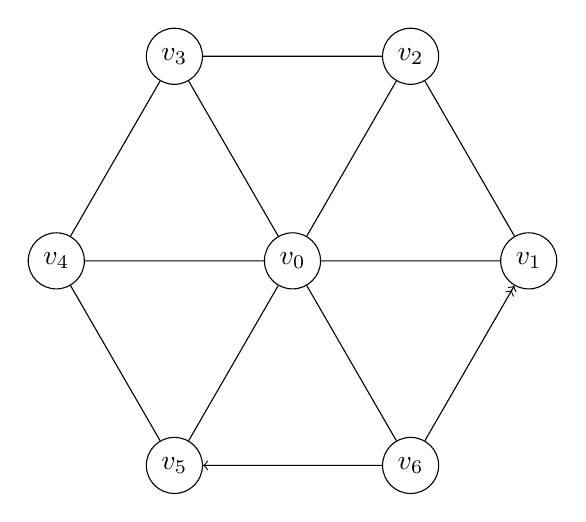
\begin{tikzpicture}
		\tikzstyle{every node}=[draw,shape=circle];
		\node (v0) at (0:0) {$v_0$};
		\node (v1) at ( 0:3) {$v_1$};
		\node (v2) at ( 60:3) {$v_2$};
		\node (v3) at (2*60:3) {$v_3$};
		\node (v4) at (3*60:3) {$v_4$};
		\node (v5) at (4*60:3) {$v_5$};
		\node (v6) at (5*60:3) {$v_6$};
		\draw 
		(v0) -- (v1)
		(v0) -- (v2)
		(v0) -- (v3)
		(v0) -- (v4)
		(v0) -- (v5)
		(v0) -- (v6)
		(v2) -- (v1)
		(v3) -- (v2)
		(v4) -- (v3)
		(v5) -- (v4)
		(v6)[->] -- (v5);
		
		\draw (v1)[<<-] -- (v6);
	\end{tikzpicture}\\
	%\textcolor{black}{Fonte: Carvalho Neto (2017)}%%\citeonline{eumesmo2017}
	\autoria{Autoria própria}
	\label{fig:}
\end{figure}


\begin{center}
	$\dfrac{\omega_s}{\omega_p}$\\ 
	\vspace{5mm}
	$\frac{\omega_s}{\omega_p}$
\end{center}



\begin{equation}
	\centering
	\dfrac{\omega_s}{\omega_p} 
	\frac{\omega_s}{\omega_p}
	\label{eq:teste}
\end{equation}

Os primeiros motores foram desenvolvidos pela empresa alemã \textit{Siemens}, que funcionava através da corrente continua. Tempos mais tarde após a descoberta da corrente alternada os motores de indução trifásica foram construídos.
Os motores de indução podem ser classificados em dois tipos: motores síncronos e assíncronos, onde o motor síncrono de corrente alternada tem como estator, eletroímãs, no qual movimenta em sincronia com a frequência da rede, que no caso do Brasil é 60 HZ, ou seja, variando a frequência da rede, varia-se proporcionalmente a velocidade do motor. Para os motores assíncronos, o mais utilizado, que corresponde a 90\% do mercado, são mais simples, consequentemente mais baratos, também é conhecido como motor de gaiola.
Para manipulação deste tipo de equipamento é importante conhecer informações como: Torque, velocidade e escorregamento, que está relacionado diretamente com as suas características de funcionamento, ou seja, a alteração de qualquer parâmetro acima citado seja através da sua fonte de alimentação, características do motor e/ou carga aplicada, pode determinar a sua forma de operação, sendo ela, eficiente ou ineficiente.
A velocidade de um motor de indução pode ser alterada durante o seu funcionamento normal de trabalho. A carga aplicada ao motor pode determinar mudanças de seu comportamento durante sua operação, sendo assim, um freio eletromagnético acoplado ao motor de indução pode proporcionar ensaios e simulações didáticas através de controles realizados pelo usuário. 

\begin{table}[!h]
	\centering
	\caption[Teste]{Valores aleatórios sem significados.}
	%\vskip 3mm
	\begin{tabular}{c|c|c|c}
		\hline
		A & B & C & D \\
		\hline
		10,00 & 54 & 54 & 74 \\
		\hline
		101,01 & R\$ 21,00 & 41 & 67 \\
		\hline
		74,03 & 85 & 96 & 21 \\
		\hline
		48,00 & 68 & 67 & 58 \\
		\hline
	\end{tabular}
	\vskip 3mm
	Fonte: Autoria própria (2021)
	\label{tab:teste}
\end{table}

Segundo \citeonline{Liu:2011} o freio eletromagnético  por correntes induzidas é desenvolvido por Wouterse em 1991, este estudo descreve que a influência do campo magnético gerado pelas correntes sobre a força de frenagem é em função da velocidade de rotação do disco \cite{Kasper:2014}.
O perfeito acoplamento do freio eletromagnético ao motor de indução proporcionará através de um controle a possibilidade de simulações de cargas, realizado através de um sistema embarcado.

Os microcontroladores, componentes essenciais nos sistemas embarcados, permitem a conexão com dispositivos analógicos e digitais, e através de circuitos simples é possível monitorar e controlar: umidade, luminosidade, velocidade, variação de campo magnético, temperatura, ou seja, infinitas possibilidades.

Diante da importância em simulação de carga para motores de indução, o trabalho proposto terá como desenvolvimento, uma bancada didática para simulação de carga em motores elétricos de indução, bem como a construção de um freio eletromagnético para acoplamento ao motor, e um controle digital para simular diversos tipos de cargas mecânicas. O conhecimento de como estes motores se comportam em campo é alvo de bastante estudos e de extrema importância para os trabalhos realizados na matéria de Maquinas Elétricas oferecidas em faculdades de Engenharia Elétrica. Os laboratórios para ensaios e simulações de cargas aplicados em motores de indução equipado com o simulador de carga para o motor de indução permitirá ao aluno maiores conhecimentos didáticos na realização de estudos e experiências práticas \cite{Liu:2011}.

\begin{citacaodireta}
	As citações diretas, no texto, com mais de três linhas, devem ser
	destacadas com recuo de 4 cm da margem esquerda, com letra menor que a do texto
	utilizado e sem as aspas. Na classe \textbf{\corujatex} recomenda-se a utilização do ambiente \textbf{citacaodireta} \cite[Pg.3]{Liu:2011}.
\end{citacaodireta}

Segundo \citeonline{Liu:2011} os microcontroladores, componentes essenciais nos sistemas embarcados, permitem a conexão com dispositivos analógicos e digitais, e através de circuitos simples é possível monitorar e controlar: umidade, luminosidade, velocidade, variação de campo magnético, temperatura, ou seja, infinitas possibilidades.
Diante da importância em simulação de carga para motores de indução, o trabalho proposto terá como desenvolvimento, uma bancada didática para simulação de carga em motores elétricos de indução, bem como a construção de um freio eletromagnético para acoplamento ao motor, e um controle digital para simular diversos tipos de cargas mecânicas. O conhecimento de como estes motores se comportam em campo é alvo de bastante estudos e de extrema importância para os trabalhos realizados na matéria de Maquinas Elétricas oferecidas em faculdades de Engenharia Elétrica. Os laboratórios para ensaios e simulações de cargas aplicados em motores de indução equipado com o simulador de carga para o motor de indução permitirá ao aluno maiores conhecimentos didáticos na realização de estudos e experiências práticas \cite{Liu:2011}.

Os microcontroladores, componentes essenciais nos sistemas embarcados, permitem a conexão com dispositivos analógicos e digitais, e através de circuitos simples é possível monitorar e controlar: umidade, luminosidade, velocidade, variação de campo magnético, temperatura, ou seja, infinitas possibilidades.
Diante da importância em simulação de carga para motores de indução, o trabalho proposto terá como desenvolvimento, uma bancada didática para simulação de carga em motores elétricos de indução, bem como a construção de um freio eletromagnético para acoplamento ao motor, e um controle digital para simular diversos tipos de cargas mecânicas. O conhecimento de como estes motores se comportam em campo é alvo de bastante estudos e de extrema importância para os trabalhos realizados na matéria de Maquinas Elétricas oferecidas em faculdades de Engenharia Elétrica. Os laboratórios para ensaios e simulações de cargas aplicados em motores de indução equipado com o simulador de carga para o motor de indução permitirá ao aluno maiores conhecimentos didáticos na realização de estudos e experiências práticas \cite{Liu:2011}.

Os microcontroladores, componentes essenciais nos sistemas embarcados, permitem a conexão com dispositivos analógicos e digitais, e através de circuitos simples é possível monitorar e controlar: umidade, luminosidade, velocidade, variação de campo magnético, temperatura, ou seja, infinitas possibilidades.
Diante da importância em simulação de carga para motores de indução, o trabalho proposto terá como desenvolvimento, uma bancada didática para simulação de carga em motores elétricos de indução, bem como a construção de um freio eletromagnético para acoplamento ao motor, e um controle digital para simular diversos tipos de cargas mecânicas. O conhecimento de como estes motores se comportam em campo é alvo de bastante estudos e de extrema importância para os trabalhos realizados na matéria de Maquinas Elétricas oferecidas em faculdades de Engenharia Elétrica. Os laboratórios para ensaios e simulações de cargas aplicados em motores de indução equipado com o simulador de carga para o motor de indução permitirá ao aluno maiores conhecimentos didáticos na realização de estudos e experiências práticas \cite{Liu:2011}.